\documentclass[a4paper,10pt]{article}
\usepackage{graphicx}
\usepackage{fancyvrb}
\usepackage{color}
\usepackage{xcolor}
\usepackage{verbatim}
\usepackage{amssymb}
\usepackage{amsmath}
\usepackage{hyperref}
\usepackage{natbib}
\usepackage{caption}
\usepackage{subcaption}

\hypersetup{urlcolor=blue, colorlinks=true} 
\usepackage{float}

%used in SL section
\usepackage{mathptmx}
\usepackage{siunitx} %SI-einheiten
\usepackage{lmodern} %weitere mathematischen Symbole
\usepackage{placeins} %floatbarrier

\DeclareSIUnit\parsec{pc}
\DeclareSIUnit\lightyear{ly}
\DeclareSIUnit\year{yr}
\DeclareSIUnit\erg{erg}
\DeclareSIUnit\ster{ster}
\DeclareSIUnit\arcsec{arcsec}
\DeclareSIUnit\deg{deg}

\definecolor{gruen}{cmyk}{0.35,0.01,0.80,0.1}

\textheight=25.5cm
\textwidth=17.5cm
\voffset=0.cm
\hoffset=-0.0cm
\oddsidemargin -1cm
\evensidemargin -1cm
\topmargin -2cm
\baselineskip=0.900cm
\setlength{\parindent}{0in}

\graphicspath{{../figures/}}

\providecommand{\e}[1]{\ensuremath{\times 10^{#1}}}
\newcommand{\given}[2]{\ensuremath{P(#1|#2)}}
\newcommand{\x}[0]{\ensuremath{\vec{x}}}
\newcommand{\gauss}[3]{\ensuremath{\frac{1}{\sqrt{2\pi#2^2}}\text{exp}\left(- \frac{(#1-#3)^2}{2#2^2}\right)}}
\newcommand{\degree}{\ensuremath{^{\circ}}}

% used in SL section
\newcommand{\todo}[2]{\textcolor{red}{\textbf{TODO (#1): #2}}}


\title{Metric Summary for GW Follow-up Target of Opportunity Visits}
\author{M. Soares-Santos, E. Neilsen}
\date{}

\begin{document}
\maketitle
This document describes a simple metric for evaluating an observing strategy for use in identifying optical counterparts to kilonovae (mergers of neutron starts) discovered using gravitational wave detectors. Currently available results from the operations simulator (OpSim) do not include triggered exposures at all, so relevant metrics cannot be applied directly.

The ultimate metric is the uncertainty on $H_0$ as measured using distances to kilonovae. This metric is related through simple statistics to the number of kilonovae identified, which in turn can be mapped to the total time which can be allocated to GW Target of Opportunity followup. So, a simpler and easier to metric is the total time an observing strategy can be interrupted for GW follow-up.

For each event, we will use one of two techniques to detect optical counterparts and distinguish them from other transients. When possible, we will attempt to detect the rising light curve. Kilonovae brighten for $\sim12$ hours after the GW detection, while other transient objects fall in brightness for most of their lifetimes. So, if we can accomplish it within 12 hours of the GW detection, we will cover the GW localization region in two passes separated by one hour. When following this strategy, exposures are only required in one filter, but both passes must be made in the same filter. In O3, the GW detector run scheduled to start in early 2019, the median localization is expected to be $\sim 23 \square\degree$, an area which can be covered by LSST in 4 pointings, corresponding to 8 visits and a total of $\sim 410$ seconds (two blocks of 205 seconds, separated by an hour) to follow up using this technique. A poorly localized ($60 \square \degree$) detection can be followed up using this technique in 16 visits and a total of $\sim 12$ minutes (two blocks of 6 minutes separated by one hour).

If it is not possible to detect the rising light curve (for example because the region is not accessible during the required time window), we will distinguish kilonovae from supernovae and other transient variable sources using the color evolution. For this, we also need two passes, but the two passes should be separated by one day, and images in two filters must be collected in each pass. A GW event with median localization will require 4 pointings, corresponding to 12 visits (4 visits in each of two filters, on two nights), taking 16 minutes total (two eight minute blocks on consecutive nights). A poorly localized ($60 \square \degree$) detection can be followed up using this technique in 32 visits and a total of 25 minutes of observing (two blocks of $\sim 13$ minutes on consecutive nights).

We can provide sample lists of events and corresponding followup exposures. Simulated runs with different fractions of time dedicated to kilonova followup can then be constructed by placing cuts on the localization of events followed up, and inserting the specified exposures into the run.

An astrophysical rate of $1500$ events $\mbox{Gpc}^{-3}$ $\mbox{yr}^{-1}$, a sensitivity volume of $0.03 \mbox{Gpc}^3$, and a detector uptime fraction of $0.8$ results in $\sim 36$ events per year. Of these, 25\% will be north of $\delta=30\degree$, and a further 10\% will be too close to the sun, so only 23 events can be followed up per year -- about one event every 2 weeks. These values are appropriate for the O3 GW detector run; future upgrades will result in a much larger volume (and so more events), and better localization (so less time will be required to follow up each event). The figure below plots the number of events followed up as a function of time dedicated using O3 localizations and event rates. 

\begin{minipage}{\columnwidth}
\centering
 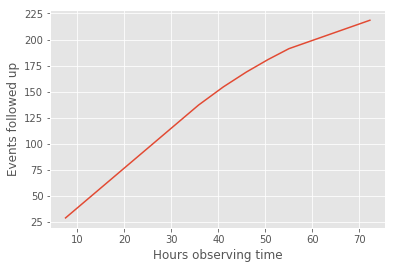
\includegraphics[width=0.5\columnwidth]{gwtoofollowupsvstime.png}
% \caption{Number of followed-up candidates as a function of observing time (hours), total for the 10 year survey assuming O3 sensitivity and localization.}
 \label{fig:followupsvstime}
\end{minipage}

%\begin{figure}
%\centering
%\includegraphics[width=\linewidth]{followupsvstime.png}
%\caption{Number of followed-up candidates as a function of observing time (hours), total for the 10 year survey assuming O3 sensitivity and localization.}
%\label{fig:followupsvstime}
%\end{figure}

\end{document}
